\documentclass[11pt, oneside]{article}   	% use "amsart" instead of "article" for AMSLaTeX format
\usepackage{geometry}                		% See geometry.pdf to learn the layout options. There are lots.
\geometry{letterpaper}                   		% ... or a4paper or a5paper or ... 
%\geometry{landscape}                		% Activate for for rotated page geometry
%\usepackage[parfill]{parskip}    		% Activate to begin paragraphs with an empty line rather than an indent
\usepackage{graphicx}				% Use pdf, png, jpg, or eps� with pdflatex; use eps in DVI mode
								% TeX will automatically convert eps --> pdf in pdflatex		
\usepackage{amssymb}
\usepackage{amsmath}
\usepackage{parskip}
\usepackage{color}

\title{Mean, variance and expectation}
%\author{The Author}
%\section{}
% \subsection*{R code}
\date{}							% Activate to display a given date or no date

\graphicspath{{/Users/telliott_admin/Dropbox/Tex/png/}}

% \begin{center} 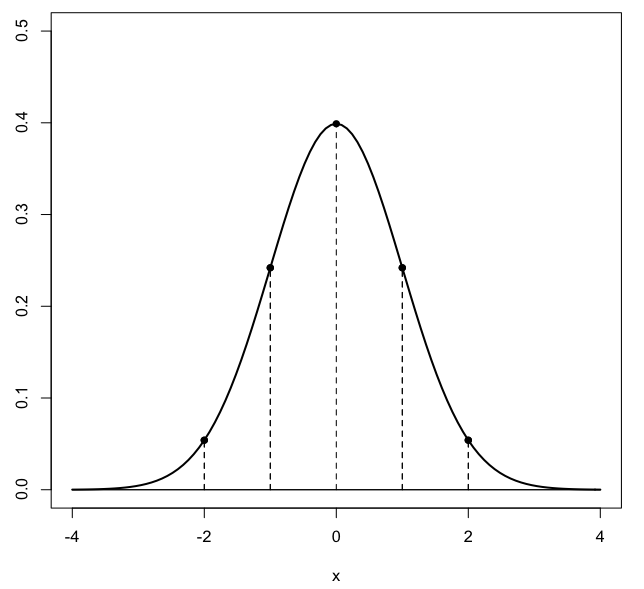
\includegraphics [scale=0.4] {gauss3.png} \end{center}
% \begin{bmatrix} a  &  b \\ c  &  d \end{bmatrix}
% \bigg |_

\begin{document}
\maketitle
\large

This short write-up is an elementary exploration of the topics listed in the title.  As you know, the mean of a bunch of numbers (say, scores on an exam) is 

\[  \frac{1}{N} ( \ x_1 + x_2 + \dots + x_N) =  \frac{1}{N} \ \sum \limits_{i=1}^N \ x_i \]

Add up all the scores $x_i$ and then divide by the total number of scores (or students), $N$, to find the mean or average value.

Alternatively, we can generate a probability distribution of scores where $C(n)$ is a \emph{count} of the number of students with a particular score $n$ and 
 
\[ P(n) = \frac{1}{N} \ C(n) \]

For example, if $5$ students take an exam, and two students score 60, two students score 70, and one student scores 100 (all answers correct), then

\[ P(60) = \frac{1}{N} C(60) =   \frac{2}{5} = P(70) = 2 P(100) \]

With this definition, $P(n)$ is normalized, having the property

\[ \sum \limits_{n=0}^{100} \ P(n) = \sum \limits_{n=0}^{100} \  \frac{1}{N} \ C(n) = \frac{1}{N} \ \sum \limits_{n=0}^{100}\ C(n) = 1 \]

Notice the limits.  Now we are summing over the different scores from $n=0 \rightarrow 100$, whereas previously we were summing over the $N$ individual scores $x_i$.

The average, mean or expected score is defined to be

\[ \langle n \rangle = \sum \limits_{n=0}^{100} \ n P(n) = \frac{1}{N} \sum \limits_{n=0}^{100} n C(n) \]

For example, if as before two students score 60, two students score 70, and one student scores 100

\[ \langle n \rangle = \sum \limits_{n=0}^{100} \ n P(n) = 60 \times \frac{2}{5} + 70 \times \frac{2}{5} + 100 \times \frac{1}{5} = \frac{360}{5} = 72 \]

Alternatively

\[ \langle n \rangle = \frac{1}{N} \sum \limits_{n=0}^{100} n C(n) = \frac{1}{5} \ (2 \times 60 + 2 \times 70 + 100) = \frac{360}{5} = 72 \]

All three views of the problem yield the same result:

\begin{itemize}
\item {add up all the scores $x_i$, and divide by $N$}
\item add up the count (how many times score $n$ occurs) multiplied by $n$ for each $n$, and divide by $N$
\item add up the probability of $n$  times $n$ for each $n$
\end{itemize}

The mean is often written like this as well:  $ \bar{x}$, when we're talking about a sum over each observed score.

In addition to the mean, the other information usually desired is the variance or standard deviation.  The variance (square of the standard deviation) can be given in terms of the scores $x_i$

\[ \sigma^2 = \frac{1}{N} \ \sum \limits_{i=1}^N \ (x_i  - \bar{x})^2 \]

In terms of counts, the equivalent calculation is

\[ \sigma^2 = \frac{1}{N} \ \sum \limits_{n=0}^{100} \ (n - \langle n \rangle)^2 C(n)  \]

and in terms of probability it's even easier:

\[ \sigma^2 =  \ \sum \limits_{n=0}^{100} \ (n - \langle n \rangle)^2 P(n)  \]

Refer to what's above in the calculation of the \emph{expected} value of $n$:

\[ \langle n \rangle = \frac{1}{N} \sum \limits_{n=0}^{100} n C(n) = \sum \limits_{n=0}^{100} \ n P(n)  \]

for the variance we have 

\[ \sigma^2 = \frac{1}{N} \ \sum \limits_{n=0}^{100} \ (n - \langle n \rangle)^2 C(n) =  \ \sum \limits_{n=0}^{100} \ (n - \langle n \rangle)^2 P(n)  \]

 so this shorthand is also correct:

\[ \sigma^2 = \langle (n - \langle n \rangle)^2 \rangle \]

Again, the reason for the $C(n)$ is that we are counting over the possible scores from $0 \rightarrow 100$, not the individual student scores.  I hope you can see those brackets clearly.  We have the expected value of an expression in parentheses, which itself is the difference between $n$ and the mean of all $n$, squared.

There is a shortcut to the calculation 

\begin{equation}
\boxed{ \sigma^2 =  \langle (n - \langle n \rangle)^2 \rangle = \langle n^2 \rangle - \langle n \rangle^2 }
\end{equation}

which we'd like to understand, but most important, remember!  We had

\[ \sigma^2 = \frac{1}{N} \ \sum \limits_{n=0}^{100} \ (n - \langle n \rangle)^2 C(n)  \]

The probability version is

\[  \sigma^2 = \ \sum \limits_{n=0}^{100} \ (n - \langle n \rangle)^2 \ P(n)  \]

Expand the square

\[ = \ \sum \limits_{n=0}^{100} \ (n^2 - 2 n \langle n \rangle + {\langle n \rangle}^2) \  P(n)  \]

breaking up the sum, and recognizing that $\langle n \rangle$ is just a constant

\[ = \sum \limits_{n=0}^{100} \ n^2 \  P(n) +  2 \langle n \rangle \sum \limits_{n=0}^{100} \  n P(n)  + {\langle n \rangle}^2   \sum \limits_{n=0}^{100} P(n)  \]

Now, the first term (which we \emph{could} write with $1/N$ out front and substituting $C(n)$

\[ \frac{1}{N} \sum \limits_{n=0}^{100} \ n^2 \  C(n) = \langle n^2 \rangle \]

is just the expectation, mean or average value of $n^2$.  And the second term is

\[ 2 \langle n \rangle \sum \limits_{n=0}^{100} \  n P(n)  = 2   \langle n \rangle   \langle n \rangle =  2 { \langle n \rangle}^2  \]

So finally, we get that 

\[  \sigma^2 = \langle n^2 \rangle - 2 { \langle n \rangle}^2 + { \langle n \rangle}^2 =   \langle n^2 \rangle -  { \langle n \rangle}^2 \]

\subsection*{coda}

Perhaps you don't like this probability stuff.  I don't blame you.  Go back to thinking in terms of individual scores:

\[ \sigma^2 = \frac{1}{N} \ \sum \limits_{x=0}^N \ (x_i  - \bar{x})^2 \]
\[ =  \frac{1}{N} \ \sum \limits_{x=0}^N \ x_i^2 - 2 x_i \bar{x} +  \bar{x}^2 \]
\[ =  \frac{1}{N} \ \sum \limits_{x=0}^N \ x_i^2 - 2\bar{x} \  \frac{1}{N} \ \sum \limits_{x=0}^N \ x_i +  \bar{x}^2 \ \frac{1}{N} \ \sum \limits_{x=0}^N  1 \]
\[ = \bar{x^2}  - 2 {\bar{x}}^2 + {\bar{x}}^2  \]
\[ = \bar{x^2}  - {\bar{x}}^2  \]

Let's just check:
\[ L = [1:10] \]
\[ \Sigma L =  1 + 2 + \dots + 10 = 55 \]
\[ \bar{x} = \frac{1}{N} \Sigma L = \frac{1}{10} 55 = 5.5 \]
\[ \bar{x}^2= 5.5^2 = 30.25 \]
\[ \bar{x^2} = \frac{1}{N} \Sigma L = \frac{1}{10} (1 + 4 + 9 + 16 + 25 + 36 + 49 + 64 + 81 + 100 = \frac{1}{10} \ 385 = 38.5 \]
\[ \sigma^2 =  38.5 - 30.25 = 8.25 \]

The standard calculation is 

\[ \sigma^2 =  \frac{1}{N} ( 2 \times {4.5}^2 + 2 \times {3.5}^2+ 2 \times {2.5}^2+ 2 \times {1.5}^2+ 2 \times {0.5}^2) \]
\[ =  \frac{1}{N} (40.5 + 24.5 + 12.5 + 4.5 + 0.5) \]
\[ =  \frac{1}{N} \ 82.5 =  \frac{1}{10} \ 82.5 = 8.25 \]

Now when I check this using R, the result is $9.16 = 82.5/9$.  There is a crucial distinction in statistics between population  measures and sample measures.  The default sample measure divides by $N-1$.  This makes no difference to any argument I've made here.

\end{document}  